\documentclass{subfiles}
\begin{document}
\section{Optimization of the Morse Double-Well Parameters}\label{sec:optimization_result}
Applying the optimization procedure outlined in Section \ref{sec:optimization_procedure}, we identify two sets of optimal parameters for the Morse double well potential that meet the desired energy and entanglement criteria. Configuration $C_I$ is tailored to yield distinct, well-separated single-particle energy spectrums and vanishing two-body entanglement, while configuration $C_{II}$ is designed to produce a significant two-body entanglement and enforce a degeneracy of the first excited single-particle energy levels in each well to enable coherent mixing of the $\ket{10}$ and $\ket{01}$ logical states.
\\ 
\begin{table}[h!]
  \centering
  \caption{Optimized Morse potential parameters for configurations \(C_1\) (separable) and \(C_2\) (degenerate).}
  \label{tab:optimized_params}
  \begin{tabular}{lcc}
    \toprule
    Parameter & $C_{I}$ & $C_{II}$ \\
    \midrule
    \(D_L\) (depth of left well)       [a.u.] & 62.1709 & 62.9733 \\
    \(D_R\) (depth of right well)      [a.u.] & 60.7336 & 64.1174 \\
    \(k_L\) (width of left well)       [a.u.] & 19.8947 & 13.2271 \\
    \(k_R\) (width of right well)      [a.u.] & 21.8194 & 13.0978 \\
    \(d\)   (inter-well separation)     [a.u.] & 15.0000 & 14.9574 \\
    \bottomrule
  \end{tabular}
\end{table}

Table \ref{tab:optimized_params} summarizes the five optimized parameters - depths of the left and right wells $D_L$ and $D_R$, widths $k_L$ and $k_R$, and inter-well separation $d$ -  for each configuration, all in atomic units (a.u.). In $C_I$ a deeper left well ($D_L = 62.1709$ a.u.) alongside a shallower right well ($D_R = 60.7336$ a.u.) ensures distinct eigenenergies and a von Neumann entanglement entropy of $S_{VN} = 0.0000$ across the first 6 energy eigenstates, indicating a product state regime. Configuration $C_{II}$, on the other hand, slightly increases the right-well depth ($D_R = 64.1174$ a.u.) and adjust a more balanced width for both wells ($k_L = 13.2271$ a.u., $k_R = 13.0978$ a.u.) so that the first excited single-particle energies coincide within numerical tolerance, and we have degeneracy in our two-particle system.

This engineered degeneracy creates a sharp 'entanglement peak' in the potential parameter space, allowing our ramp protocol to traverse from $C_I$ to $C_{II}$ to induce mixing of the logical states $\ket{10}$ and $\ket{01}$, and thus, generate a significant two-body entanglement. The two configurations are similar within a few atomic units, so quantum control protocols can perturb our system without having to significantly alter the system architecture, with minimal control overhead.
\begin{figure}[h!]
  \centering
  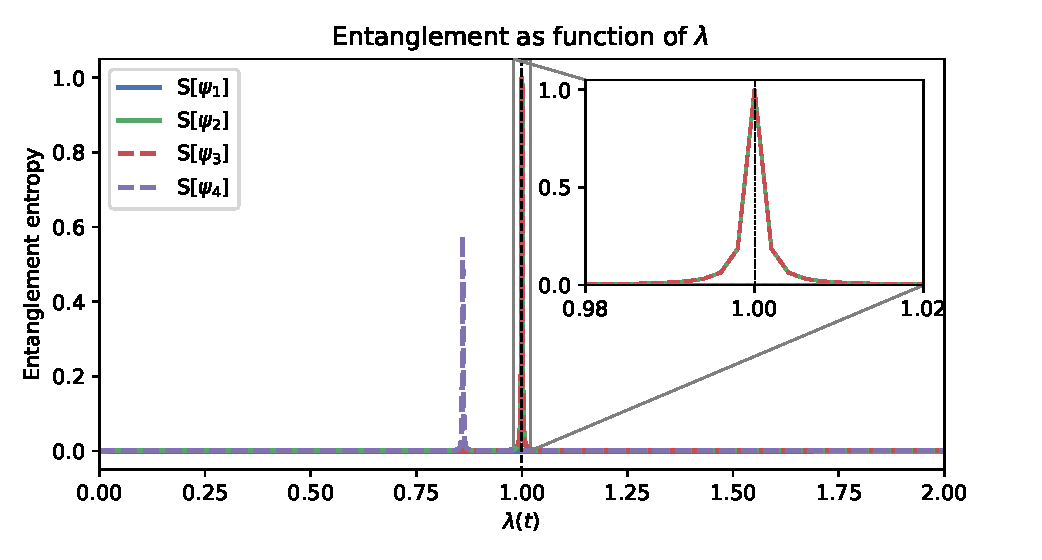
\includegraphics[width=1.0\textwidth]{figs/entanglement_peak.pdf}
  \caption{The entanglement peak in the parameter space of the Morse double-well potential. The plot shows the von Neumann entanglement entropy $S_{VN}$ in the first four eigenstates of the system, as a function of sweeping parameter $\lambda(t)$. The inset highlights the sharpness of the peak, indicating a narrow range of parameters where the first excited states are nearly degenerate, allowing for significant two-body entanglement generation. The peak is centered around $\lambda = 1$, corresponding to configuration $C_{II}$, where the first excited states are entangled. Parameters for configuration $C_I$ and $C_{II}$ are listed in Table \ref{tab:optimized_params}}. 
  \label{fig:entanglement_peak}
\end{figure}
Figure \ref{fig:entanglement_peak} illustrates the sharpness of the entanglement peak in the parameter space of our optimization procedure. The plot shows the von Neumann entanglement entropy $S_{VN}$ in the first four eigenstates of the system, as a function of sweeping parameter $\lambda(t)$ as we traverse from configuration $C_I$ at $\lambda = 0$, to configuration $C_{II}$ at $\lambda = 1.0$ and beyond. The inset highlights the sharpness of the peak where we have 'good' parameters that allow for significant two-body entanglement generation. This illustrates the difficulty of optimizing the parameters for configuration $C_II$, as the parameter space is barren and mostly flat (it looks more flat in the figure due to the sweep being linear, as seen in \eqref{eq:interpolation_function}), and why a good initial guess was crucial for the optimization procedure to converge to the desired configuration.

\begin{figure}[h!]
  \centering
  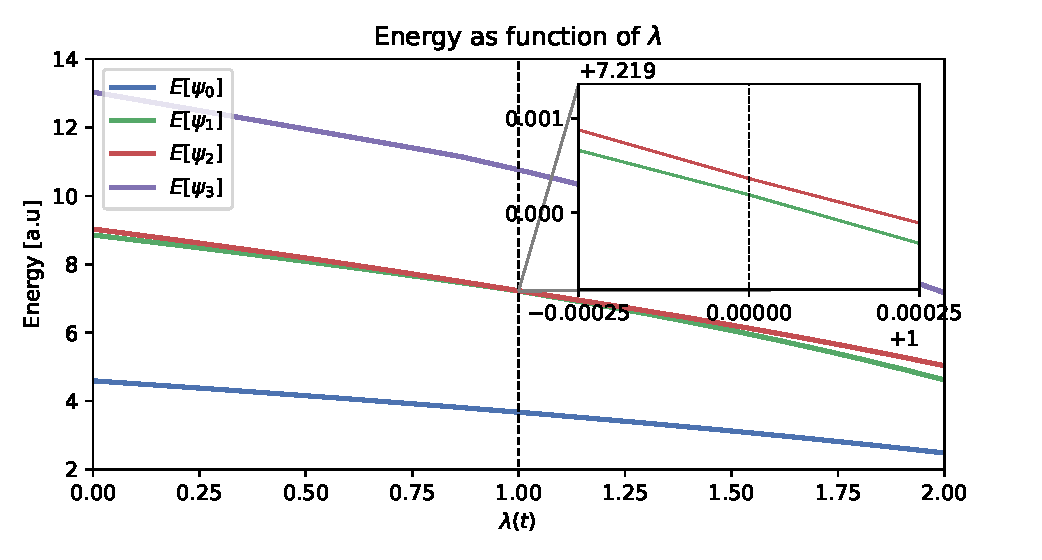
\includegraphics[width=1.0\textwidth]{figs/energy_curves_avoided_crossing.pdf}
  \caption{Energy curves for the four lowest lying energy eigenstates of the Morse potential as a function of ramping parameter $\lambda(t)$. The curves illustrate the avoided crossing between the first excited states in configuration $C_{II}$, where the first excited states $\ket{10}$ and $\ket{01}$ are nearly degenerate, and repel each other. The inset highlights the avoided crossing, where the non-interacting energies would cross and 'swap' places, but due to the Coulomb interaction the states repel each other, creating a 'gap' in the energy spectrum. Because our numerical procedure only enforces near-degeneracy, we omit overlaying the non-interacting energies to avoid confusion, as they are shifted in the spectrum due to the degeneracy not being exact. }
  \label{fig:energy_curves_avoided_crossing}
\end{figure}
In the inset of figure \ref{energy_curves_avoided_crossing} we show the avoided crossing of the first excited energy levels as we move into the (near)-degenerate configuration $C_{II}$. The energy curves are plotted as a function on ramping paramter $\lambda(t)$, which varies from $0$ to $1$ as we ramp from configuration $C_I$ to $C_{II}$. The first excited states $\ket{10}$ and $\ket{01}$ are nearly degenerate, and repel each other due to the Coulomb interaction, creating a 'gap' in the energy spectrum where the non-interacting energies would cross and 'swap' places. This is akin to the avoided crossing we visualized in the Landau-Zener model in Section \ref{sec:avoided_crossings}. We originally intended to overlay the corresponding non-interacting energies (that would cross in the absence of coupling), but in practice they do not cross exactly at $\lambda = 1.0$ as our numerical procedure only enforces near-degeneracy up to finite tolerance. To avoid confusion by introducing a non-interacting energy that does not cross exactly at the same point, we omitted the non-interacting curves. We simply note that, in an ideal scenario, the uncoupled energies would indeed cross at $\lambda = 1.0$, and the avoided crossing would be exact when coupling is introduced. In our case however, the near-degeneracy is more than sufficient to induce the desired mixing of the logical states $\ket{10}$ and $\ket{01}$, and thus, generate significant two-body entanglement.
\\

\begin{figure}[h!]
  \centering
  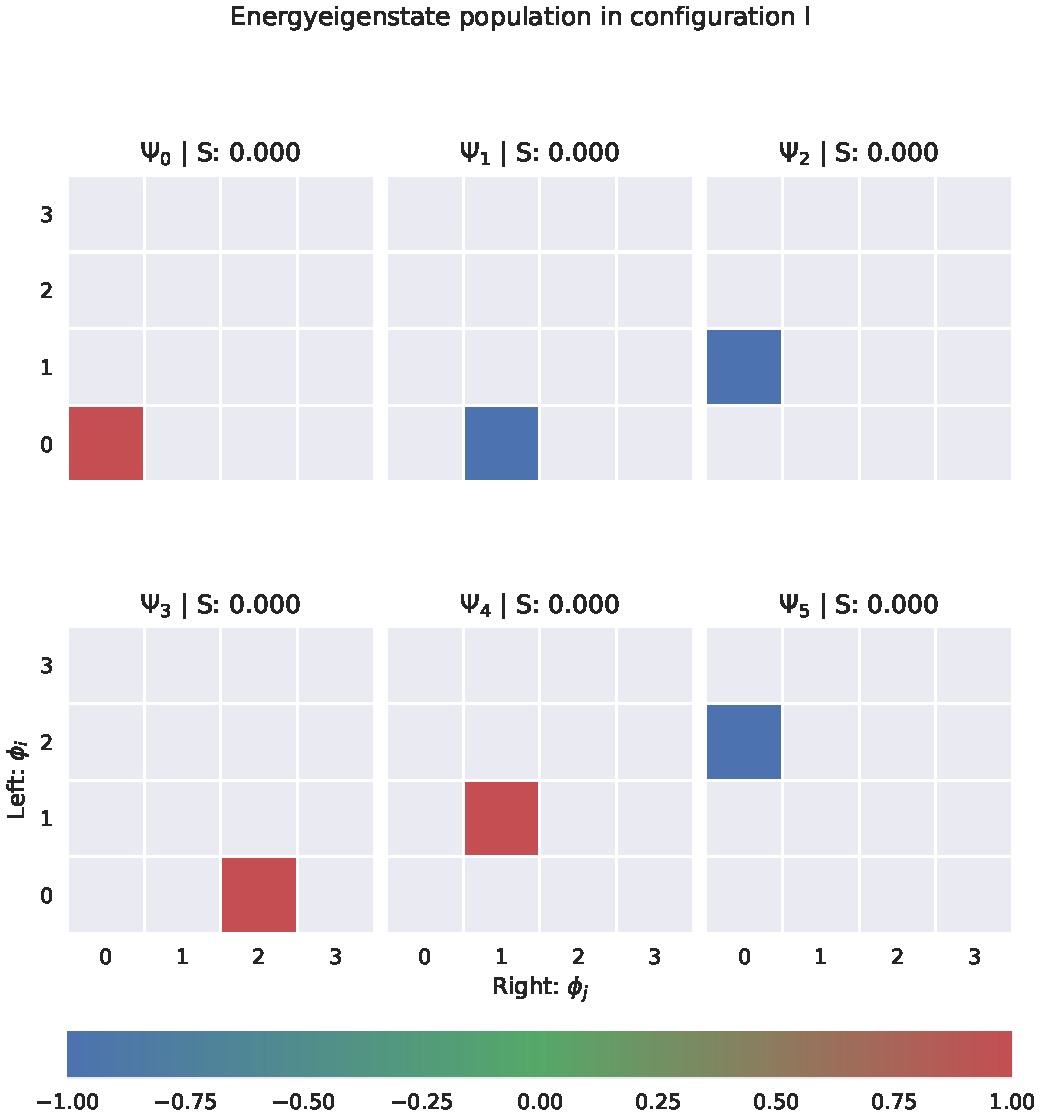
\includegraphics[width=\textwidth]{figs/state_populations_I.pdf}
  \label{fig:populations_I}
  \caption{State populations of the six lowest two-particle energy eigenstates in configuration $C_I$. Each energy eigenstate is occupied by a single computational basis state (Hartree state), and are pure product states. The entropy $S$ for each state is zero, indicating no entanglement.}
\end{figure}
Figure \ref{fig:populations_I} show the computational basis state (Hartree states) occupancy of the six lowest two-particle energy eigenstates for configuration $C_I$, where we observe that the states are indeed pure product states within a numerical tolerance of $10^{-7}$. Each eigenstate has exactly one dominant block, and is zero elsewhere - meaning the there is vanishing two-body entanglement between the particles, as seen from the listed entropy $S$ for each state - just what we aimed to achieve for the separable configuration. 
\\

\begin{figure}[h!]
  \centering
  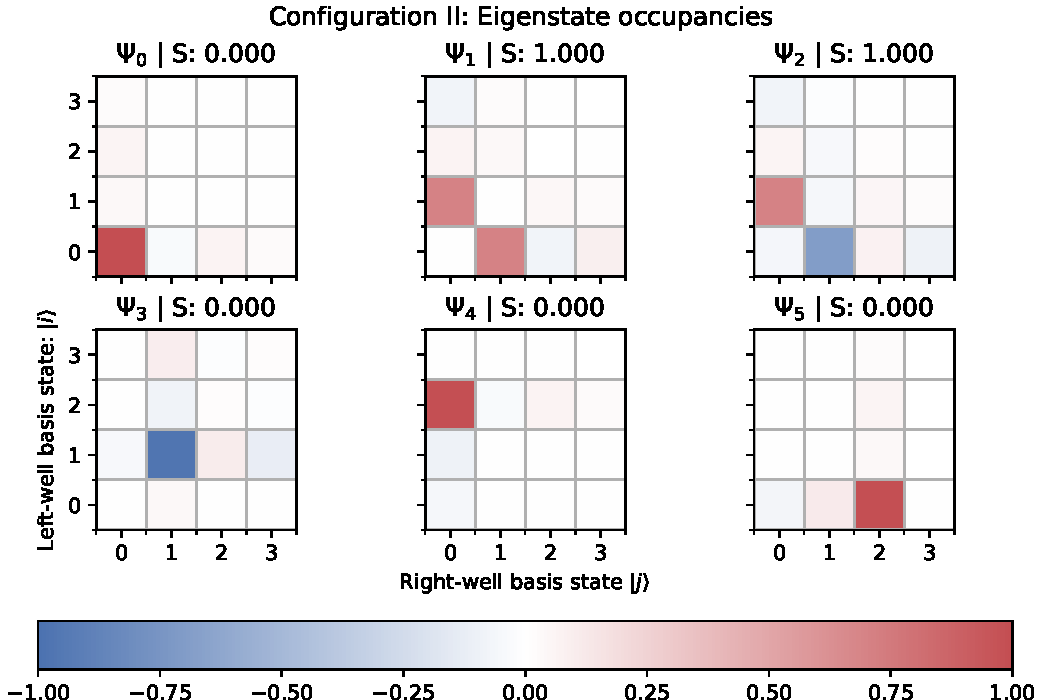
\includegraphics[width=\textwidth]{figs/state_populations_II.pdf}
  \label{fig:populations_II}
  \caption{State populations of the six lowest two-particle energy eigenstates in configuration $C_{II}$. The first excited states $\ket{10}$ and $\ket{01}$ are now mixed, with significant contributions from the first excited state in each well. The entropy $S$ for these states is equal to 1 (within a tolerance of $10^-6$), indicating (near) maximal entanglement. We note that maximal entanglement is not equivalent to being in a Bell state, but rather, maximally entangled with \emph{multiple} states beyond $\ket{01}, \ket{10}$. In this mixed configuration however, we see traces of other basis states leaking into our previously pure product states, especially prevalent in the higher energy states. This is seen as transparent red/blue tint in the heatmap, indicating minor contributions from other basis states.}
\end{figure}

By contrast, Figure \ref{fig:populations_II} illustrates the same six two-particle energy eigenstates under configuration $C_{II}$, where we observe that the first excited states $\ket{10}$ and $\ket{01}$ are now mixed, with both states having significant contributions from both wells. The mixture is almost equal, and we are close to achieve the Bell states (maximally entangled states) for these two energy eigenstates, as indicated by the entropy $S \approx 1$. This means we have near perfect superpositions of the logical states $\ket{10}$ and $\ket{01}$. The remaining states remain essentially pure product states up to numerical tolerance ($10^{-7}$), highlighting that only the desired qubit subspace is affected by the entanglement, while the rest of the two-particle Hilbert space remains unaffected. This will be crucial for quantum control protocols we aim to run. The minor contributions from other basis states, seen as transparent red/blue tint in the heatmap, are negligible, and do not significantly affect the entanglement properties of the first excited states. As long as the coupling terms are small enogh and energy gaps wide in comparison, the mixing of higher order states will not lead to unwanted transitions or decoherence in our two-qubit gate operations.
\\

Together, these two static heatmaps validate our optimization procedure: Configuration $C_I$ produces well-separated, pure energy eigenstates (pure in the sense they are singly occupied by a logical state), while configuration $C_{II}$ enforces a degeneracy of the first excited states, enabling a coherent mixing of the logical states $\ket{10}$ and $\ket{01}$, thus generating significant two-body entanglement needed for our two-qubit gate operation protocols.


These two parameter configurations form the foundation for all subsequent static analyses and dynamical simulations in the thesis work when working in the $l=4$ regime. The inter-well separation $d$ is set to $\approx 15.0$ a.u. for both configurations, which is sufficiently large to ensure negligible exchange interaction between the particles, as confirmed in Section \ref{sec:exchange_interaction}. This also is within working ranges for quantum dots, and translated into effective mass units (for GaAs) the separation corresponds to approximately $d \approx 150$ nm, which is a reasonable distance for quantum dot systems \cite{garcia2021semiconductor}, ref. the discussion in Appendix \ref{app:appendix_A} for the conversion from atomic units to effective mass units. In regular units, we note that this separation is very small compared to the typical length scales of qubit architectures, $15 a_0 \approx 0.79$ nm, one order of magnitude below the typical inter-dot separation in quantum dot systems, which is on the order of 10 nm \cite{garcia2021semiconductor}. 
\end{document}